\section{Zielsetzung}

In diesem Versuch sollen die Suszeptibilitäten verschiedener paramagnetischer Seltener-Erde-Verbindungen untersucht werden.

\section{Theorie}
\label{sec:Theorie}

In Materie setzt sich die magnetische Flussdichte $\vec{B}$ sowohl aus der magnetischen Feldstärke $\vec{H}$, wie auch der Magnetisierung $\vec{M}$ zusammen.
Dabei gilt die Relation 

\begin{equation}
    \label{eqn:mag-allg}
    \vec{B} = \mu_0 \vec{H} + \vec{M},
\end{equation}

wobei $\mu_0$ die magnetische Feldkonstante. 
Die Magnetisierung wird durch die magnetischen Momente in der Materie hervorgerufen und hängt nach 

\begin{equation}
    \label{eqn:magnetisierung}
    \vec{M} = \mu_0 \chi \vec{H}
\end{equation}

ebenfalls von der Feldstärke ab.
Dabei ist $\chi$ die sogenannte magnetische Suszeptibilität. Diese hängt sowohl von dem Material, von $\vec{H}$, als auch von der Temperatur $T$ ab.
Diese sorgt für Änderungenen in der Orientierung der Dipolmomente im Material.

An dieser Stelle sei gesagt, dass der hier zu untersuchende Paramagnetismus, im Gegensatz zum Diamagnetismus, nicht bei jedem Material auftritt.
Dies liegt daran, dass ersterer nur zu finden ist, wenn die Atome im Material einen endlichen Drehimpuls besitzen.

Im einem Atom liegen einerseits die Spins der Elektronen $\vec{S}$ und deren Bahndrehimpulse $\vec{L}$ vor.
Dies setzt sich additiv zum Gesamtdrehimpuls $\vec{J}$ zusammen.
Damit sind die Dipolmomente durch

\begin{align}
    \vec{\mu}_\text{L} &= - \frac{\mu_\text{B}}{\hslash} \vec{L} \\
    \vec{\mu}_\text{S} &= - g_\text{S} \frac{\mu_\text{B}}{\hslash} \vec{S}
\end{align}

gegeben, wobei $\mu_\text{B}$ das Bohr'sche Magneton und $g_\text{S}$ das gyromagnetische Verhältnis ist.

\begin{figure}
    \centering
    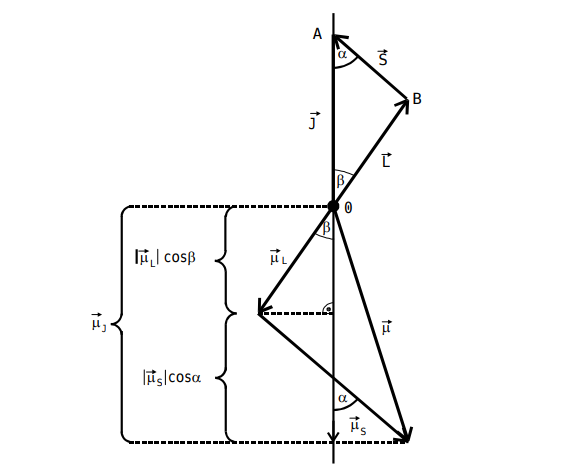
\includegraphics[width=0.70\textwidth]{content/skizze-drehimpuls.png}
    \caption{Skizze zur Vektoraddition der Drehimpulse und der magnetischen Momente im Atom \cite{V606}.}
    \label{fig:skizze-dreh}
\end{figure}

Des Weiteren liefert die Quantenmechanik für die Beträge von $\vec{L}$, $\{vec{S}$ und $\vec{J}$ die Relationen

\begin{align} 
    |\vec{L}| = L &= \sqrt{ L ( L + 1 ) } \hslash \\
    |\vec{S}| = S &= \sqrt{ S ( S + 1 ) } \hslash \\
    |\vec{J}| = J &= \sqrt{ J ( J + 1 ) } \hslash.
\end{align}

Mit den Winkelbeziehungen in \autoref{fig:skizze-dreh} und der Näherung $g_\text{S} = 2$ lässt sich das magnetische Moment zum Gesamtdrehimpuls als

\begin{equation}
    \label{eqn:magn-moment}
    \mu_\text{J} = g_\text{J} \cdot \mu_\text{B} \sqrt{J (J + 1)}
\end{equation}

schreiben, wobei 

\begin{equation}
    \label{eqn:lande}
    g_\text{J} := \frac{ 3 J (J+1) + S(S+1) - L(L+1) }{ 2 J (J +1) }
\end{equation}

der Landé-Faktor ist.
Des Weiteren kann die Richtung von $\vec{\mu}_\text{J}$ nicht beliebig sein. Für die $z$-Komponente ergibt sich

\begin{equation}
    \label{eqn:mu-z}
    \mu_\text{J, z} = - \mu_\text{B} g_\text{J} m,
\end{equation}

wobei $m \in \{ -J, J+1, ... , J-1, J \}$ die magnetische Quantenzahl ist.
Also gibt es eine diskrete Menge von möglichen Winkeln, welche jeweils eine potentielle Energie innehaben.
Mit dieser kann die Magnetisierung bestimmt werden.
Dazu wird die Häufigkeit des Auftretens der einzelnen Orientierungen berechnet und mit dem entsprechenden mangetischen Moment multipliziert.
Diese Werte werden anschließend aufsummiert.

Damit kann die Suszeptibilität über

\begin{equation}
    \label{eqn:suszep}
    \chi = \mu_0 \mu_\text{B}^2 g_\text{J} \frac{N J (J + 1)}{3 k T}
\end{equation}

beschrieben werden.
Dabei ist $k$ die Boltzmann-Konstante und $N$ die Anzahl der magnetischen Momente pro Volumeneinehit.

Bei Atomen der Seltenen Erden sind in der 4f-Schale die Elektronen so angeordnet, dass diese einen endlichen Drehimpuls liefern.
Daher lässt sich bei diesen Elementen der Paramagnetismus gut beobachten.
Diese Anordnung und der zugehörige Gesamtdrehimpuls lässt sich mit den Hund'schen Regeln beschreiben:

1. Die einzelnen Spins $\vec{s}_\text{i}$ kombinieren sich so nach dem Pauli-Prinzip, dass der Gesamtspin $\vec{S} = \sum \vec{s}_\text{i}$ maximal wird.

2. Die einzelnen Bahndrehimpulse $\vec{l}_\text{i}$ ordnen sich so an, dass der Gesamtdrehimpuls $\vec{L} = \sum \vec{l}_\text{i}$ maximal wird und zugleich Regel 1 und dem Pauli-Prinzip folgen.

3. Der Gesamtdrehimpuls ergibt sich zu $\vec{J} = \vec{L} + \vec{S}$, sollte die Schale mehr als halb gefüllt sein, beziehungsweise zu $\vec{J} = \vec{L} - \vec{S}$, wenn sie weniger als zur Hälfte gefüllt ist.



\begin{figure}
    \centering
    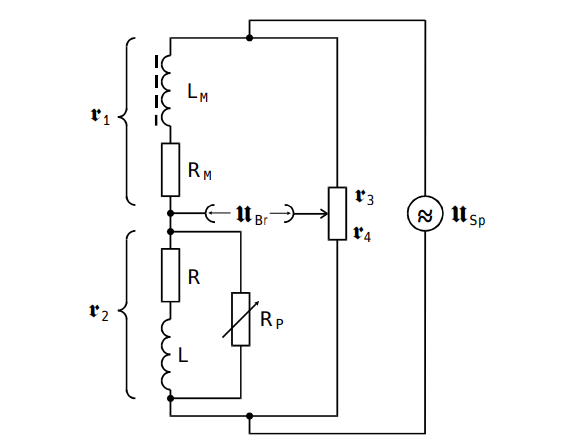
\includegraphics[width=0.70\textwidth]{content/bruecke.png}
    \caption{Schaltskizze der Brückenschaltung, welche zur Suszeptibilitätsmessung verwendet wird \cite{V606}.}
    \label{fig:bruecke}
\end{figure}

Zur experimentellen Bestimmung der Suszeptibilität wird eine Brückenschaltung, wie in \autoref{fig:bruecke} zu sehen, verwendet.
Jene beruht auf einer Induktivitätsdifferenz zwischen einer mit Luft und einer mit Material gefüllten Spule.
Daher müssen die beiden Induktivitäten der beiden Spulen möglichst gleich sein.

Zur Bestimmtun der Differenz können zwei Methoden verwendet werden.
Für die erste wird die Brücke abgeglichen, sodass $U_\text{Br} = 0$ gilt.
Wenn nun ein Material in eine der beiden Spule geschoben wird, so ändert sich die Spannung der Brücke, sodass daraus $\chi$ bestimmt werden kann.
Dabei zeigt sich nach diversen Umformungen, dass für $\omega^2 L^2 >> R^2$, die Relation
%TODO sehr viel größer als

\begin{equation}
    \label{eqn:suszep-spannung}
    \chi = 4 \frac{F U\text{Br}}{Q U_\text{Sp}}
\end{equation}

gilt, wobei $F$ der Querschnitt der Spule und $Q$ der der Probe und $U_\text{Sp}$ die Speisespannung.

Für die zweite Methode wird nach dem Einführen des Materials die Brücke erneut abgeglichen.
Aus der Differenz der Widerstände $\Delta R$, welche zum Abgleichen nötig sind, kann mittels

\begin{equation}
    \label{eqn:suszep-wider}
    \chi = 2 \frac{F \cdot \Delta R}{R_3 Q}
\end{equation}

die Suszeptibilität bestimmt werden. Dabei ist $R_3$ der Widerstand am Potentiometer.